\documentclass[12pt]{article}
\usepackage{fullpage}
\usepackage{amsmath}
\usepackage{multirow}
\usepackage{graphicx}
\usepackage{indentfirst}
\title{\LARGE \textbf{Trábajo práctico 1}}
\author{Franco Ferretti, Martín Rossi}
\date{}
\begin{document}
\maketitle
\subsection*{11.84}
\subsubsection*{a)}
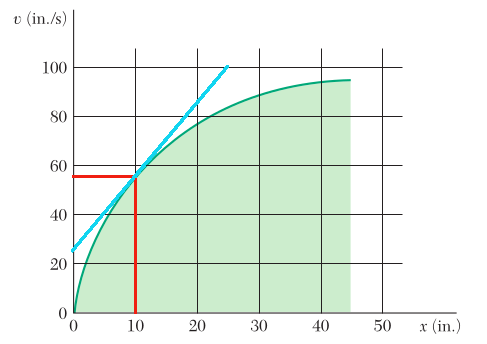
\includegraphics[width=320px]{1184a}

En el punto $x=10in$, la velocidad es aproximadamente $v=56in/s$. Se traza la pendiente en ese punto y se obtiene el segmento que va desde $(0,26)$ hasta $(25,100)$. El gráfico no usa la misma escala para el eje $x$ e $y$, la pendiente no tendrá ese ángulo pero estos dos puntos siguen siendo los mismos. El vector correspondiente a la pendiente sería $(25,74)$, y su vector normal $(74,-25)$.

Ahora se busca el punto punto $(C,0)$ tal que $(10,56)+\alpha(74,-25)=(C,0)$

$56+\alpha*-25=0 \implies \alpha=56/25=2.24$

$C=10+\alpha*76=10+2.24*76=186$

Por lo tanto $a=186-10=176in/s^2$
\subsubsection*{b)}
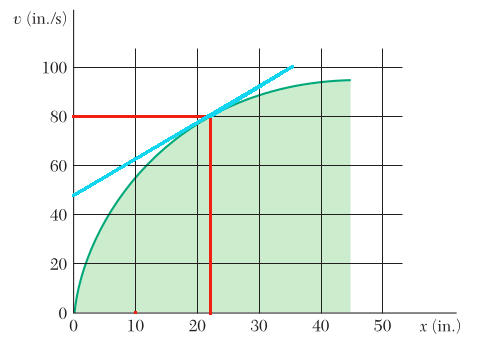
\includegraphics[width=320px]{1184b}

Se hace lo mismo para $v=80in/s$, donde $x$ es aproximadamente $22in$. La pendiente va desde $(0,50)$ hasta $(35,100)$, el vector $(35,50)$ y la normal $(50,-35)$.

$(22,80)+\alpha(50,-35)=(C,0)$

$80+\alpha*-35=0 \implies \alpha=80/35=2.28$

$C=22+\alpha*50=22+2.28*50=136$

$a=136-22=124in/s^2$
\subsection*{11.80}
$D=1.6mi=8448ft$

$-4ft/s^2\le a\le 4ft/s^2$

$-0.8ft/s^3\le \frac{\delta a}{\delta t}\le 0.8ft/s^3$

$0\le v\le 20mi/h=\frac{88}{3}ft/s$
\subsubsection*{a)}
Para llegar lo más rápido posible el tren deberá ir a su rapidez máxima de $\frac{88}{3}ft/s$ el mayor tiempo que pueda.

Como parte del reposo deberá ir aumentando su velocidad hasta llegar al máximo. Para eso tiene que acelerar, pero esa aceleración no puede variar más de $0.8ft/s^2$ por segundo.

Entonces la aceleración va a ir subiendo hasta cierto punto, y después va a bajar hasta 0 dejando al tren en la velocidad máxima. El tren recorre una distancia en velocidad máxima y después para frenarlo hace el proceso inverso.

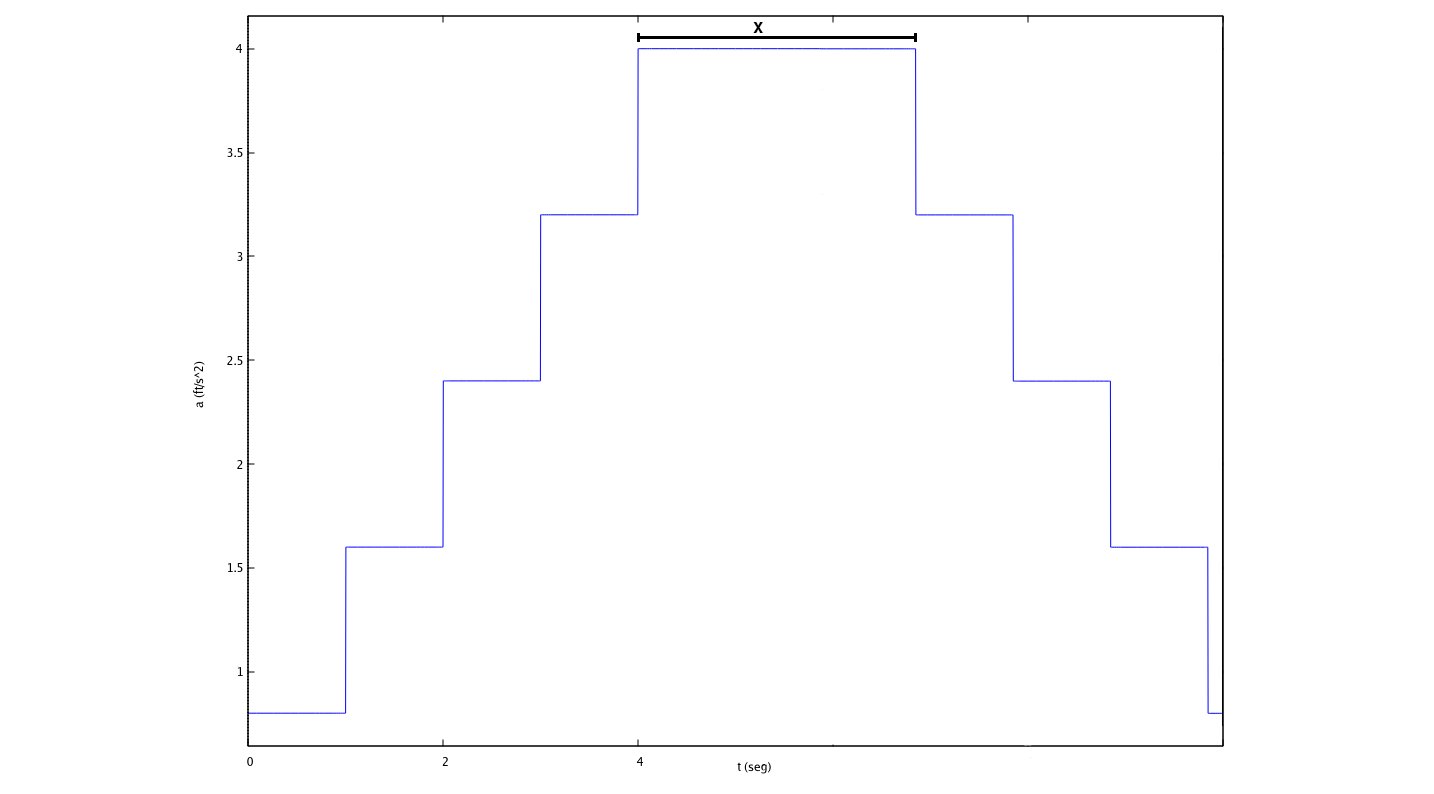
\includegraphics[width=\linewidth]{1180a}

El área bajo la curva de aceleración es igual a la velocidad, y como se sabe la velocidad máxima se busca el tiempo con la siguiente ecuación:
\begin{align*}
  0.8+1.6+2.4+3.2+4x+3.2+2.4+1.6+0.8&=\frac{88}{3}\\
  0.8(20+5x)&=\frac{88}{3}\\
  x&=\frac{10}{3}
\end{align*}

El tren tarda $\frac{10}{3}+8=\frac{34}{3}s$ en llegar a la velocidad máxima, y recorre $\frac{440}{3}ft$. Hará la misma distancia para bajar después hasta 0 de nuevo.

Entonces le faltan $8448-2*\frac{440}{3}=\frac{24464}{3}ft$ a $\frac{88}{3}ft/s$, que lo hace en $278s$.

Por lo tanto tarda $2*\frac{34}{3}+278=\frac{902}{3}\approx 300.6s=5.01min$.
\subsubsection*{b)}
La velocidad promedio es distancia sobre tiempo: $\frac{8448}{\frac{902}{3}}=\frac{1152}{41}ft/s=19.15mi/h$.
\newpage
\subsection*{11.160}
Cálculo de las componentes normales de la aceleración de los satélites con $a_n=g(R/r)^2$:

$a_A=9.8(\frac{3960}{3960+120})^2=9.23m/s^2$

$a_B=9.8(\frac{3960}{3960+200})^2=8.88m/s^2$\\

Conversión de millas a metros:

$3960+120=4080mi=6566124m$

$3960+200=4160mi=6694871m$\\

Cálculo de la velocidad tangencial con $a_n=\frac{v^2}{\rho}$:

$9.23=\frac{v_A^2}{6566124}\implies v_A=7784.94m/s$

$8.88=\frac{v_B^2}{6694871}\implies v_B=7710.41m/s$\\

Circunferencia de las órbitas:

$C_A=(2\pi*6566124)m\approx 41256173m$

$C_B=(2\pi*6694871)m\approx 42065115m$\\

El satélite A tarda $\frac{41256173}{7784.94}\approx 5300s$ en dar una vuelta. B $\frac{42065115}{7710.41}\approx 5456s$

Entonces las velocidad angular son $\omega_A=\frac{360}{5300}=\frac{18}{265} grado/s$ y $\omega_B=\frac{360}{5456}=\frac{45}{682} grado/s$\\

Hay que buscar el mínimo $t$ tal que $\frac{18}{265}t=\frac{45}{682}t$ pero módulo 360 para ver en qué ángulo se vuelven a encontrar.

$\frac{18}{265}t=\frac{45}{682}t\iff\frac{351}{18730}t=0$

Es decir que $\frac{351}{18730}t$ es múltiplo de 360. Por lo tanto $t=\frac{7229200}{39}$.\\

Hasta que se vuelvan a alinear van a tardar $\frac{7229200}{39}\approx 185364.10s=51.49h$
\end{document}